\documentclass{report}
\usepackage{graphicx} % Required for inserting images
\usepackage[italian]{babel}
\usepackage{tikz}
\usepackage{hyperref}
\usepackage{amsmath}
\usepackage{xcolor}
\usepackage{float}
\usepackage{soul}
\usepackage{listings} % Per evidenziare il codice

\definecolor{lightgray}{rgb}{0.9,0.9,0.9} % Definizione colore sfondo
\definecolor{darkgreen}{rgb}{0.0, 0.5, 0.0}

\lstset{
    backgroundcolor=\color{lightgray}, % Sfondo grigio
    basicstyle=\ttfamily, % Font monospaziato
    % frame=single, % Bordo attorno al codice
    tabsize=4, % Dimensione tabulazione
    breaklines=true, % Permette di andare a capo automaticamente
    numbers = left,
    numberstyle=\small\color{gray}
}

\title{\huge\textbf{{Integrità delle Query}}}
\date{Parte II}

\begin{document}

\maketitle

\tableofcontents
\newpage

\chapter{Integrità della computazione}

Nel nostro scenario di riferimento potremo avere più \textit{data owner}; queste 
sono entità di cui ci fidiamo.

\noindent Il problema è che questi dati potrebbero essere affidati a dei \textit{cloud provider} esterni, e che possano essere soggetti a delle \textit{computazioni};
questo potrebbe essere un problema sia in termini di confidenzialità che in termini di \textbf{integrità}: 
\textit{"chi mi dice che la tua computazione sia integra?"}.

\section{Esempi}

\subsubsection{Esempio di una query}

Abbiamo l'owner che affida i propri dati ad un provider esterno;
abbiamo poi un client che effettua una query.

\begin{figure}[H]
    \centering
    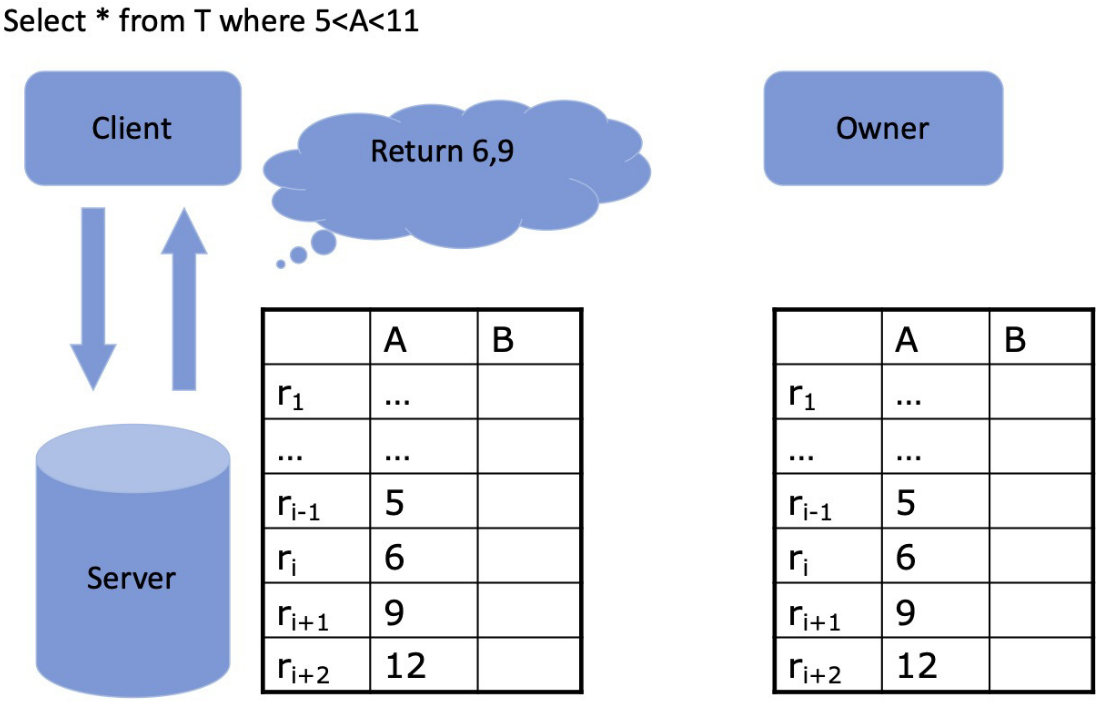
\includegraphics[width=0.7\linewidth]{images/ex1.png}
\end{figure}

\subsubsection{Esempio di query: iniezione}

Viene iniettata un'informazione fasulla; \textit{magari mi 
conviene dirti una cosa piuttosto che un'altra, le tue azioni dipendono 
da quello che ti dico\dots}

\begin{figure}[H]
    \centering
    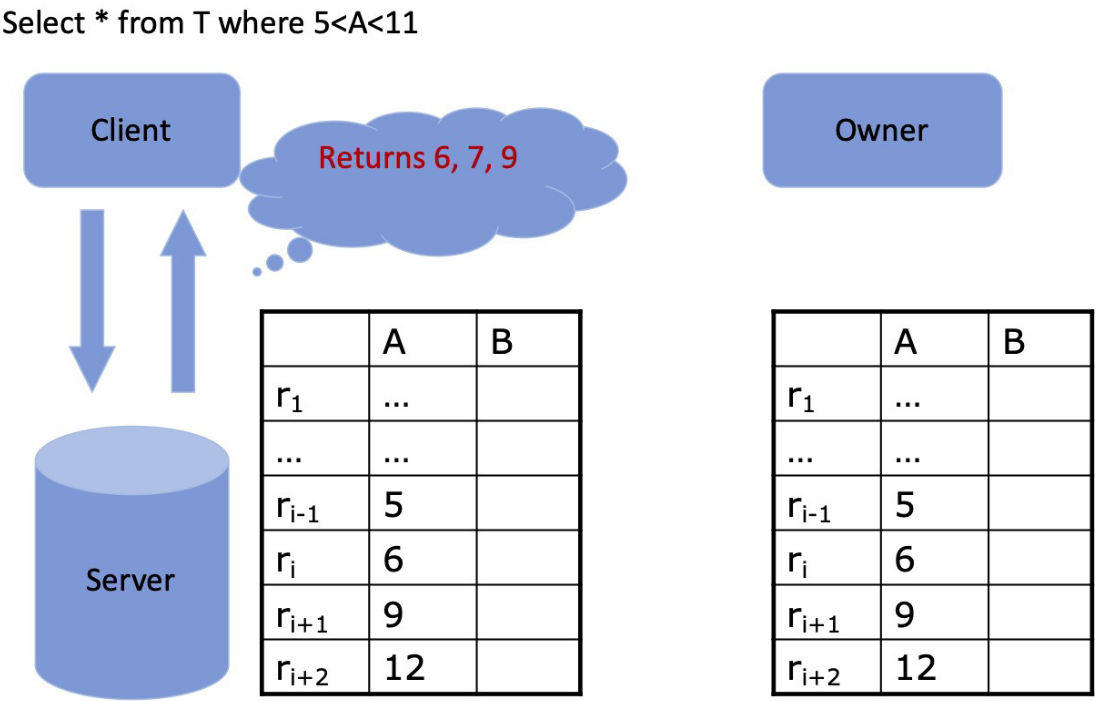
\includegraphics[width=0.9\linewidth]{images/ex2.png}
\end{figure}


\subsubsection{Esempio di query: drop}

\begin{figure}[H]
    \centering
    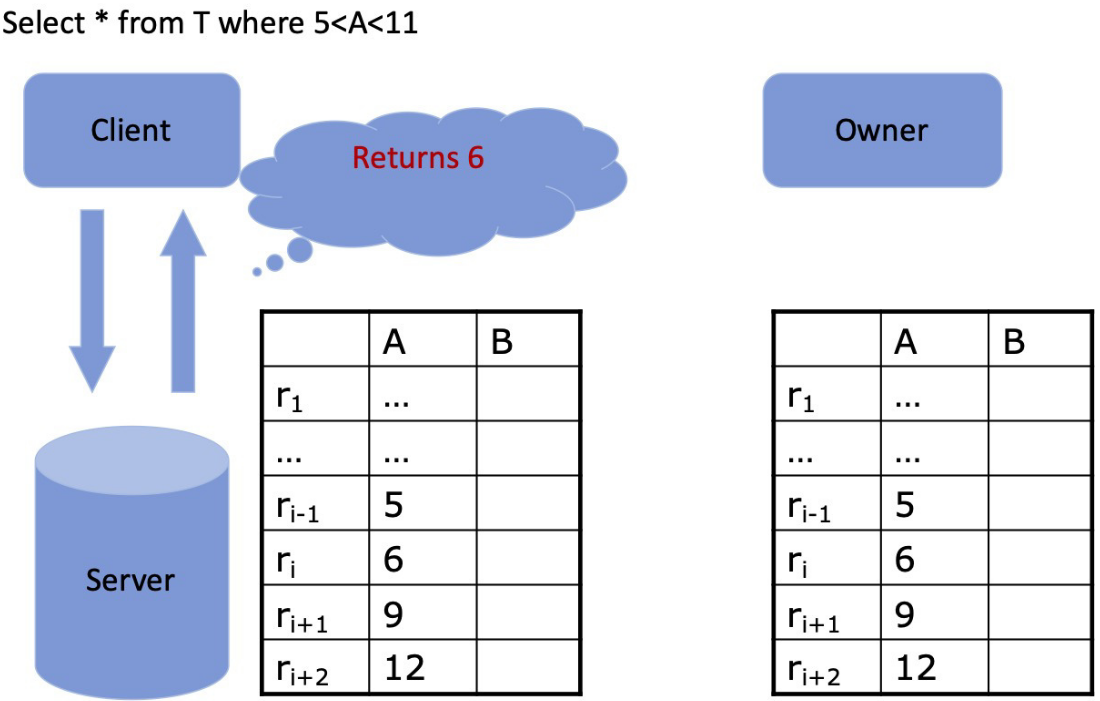
\includegraphics[width=0.9\linewidth]{images/ex3.png}
\end{figure}


\newpage
\subsubsection{Esempio di query: omissione}

I dati potrebbero essere dinamici, dunque potrebbero 
essere richieste delle operazioni di update.

\begin{figure}[H]
    \centering
    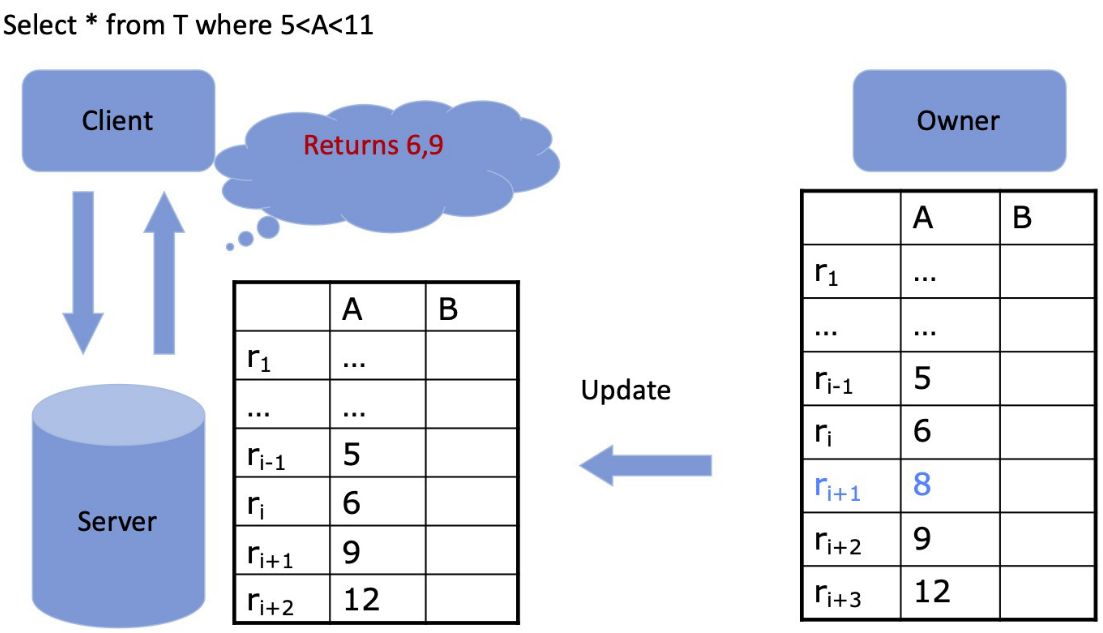
\includegraphics[width=0.9\linewidth]{images/ex4.png}
\end{figure}

\section{Integrità di storage e computazione}

Il data owner e gli utenti necessitano di meccanismi che assicurino l'integrità dei risultati 
delle query. Una query è integra se rispetta:
\begin{itemize}
    \item \textbf{Correttezza:} il risultato viene calcolato sui dati veri dell'owner (primo esempio)
    \item \textbf{Completezza:} il risultato calcolati su tutti i dati (secondo esempio)
    \item \textbf{Freschezza:} il risultato è calcolato sull'ultima versione dei dati che l'owner 
    ha dato (terzo esempio)
\end{itemize}


\noindent Ci sono due diversi tipi di approcci per rispondere al problema di integrità, 
ciascuno con i suoi vantaggi e svantaggi:
\begin{itemize}
    \item \textbf{Deterministico:} \textit{se il risultato di una computazione è integro, sono sicuro 
    al 100\% che sia integro}

    \noindent Queste tecniche vengono implementate in modo che l'owner dà al provider, oltre ai 
    dati da gestire, anche delle strutture ausiliarie che vengono sfruttate per verificare l'integrità della computazione 
    \item \textbf{Probabilistico:} \textit{ti dico sempre se è integro o no, ma non con certezza 
    assoluta ma con una certa probabilità; c'è della probabilità di fare degli errori}

    \noindent Perché si usano questi approcci? Sono tecniche che hanno lo svantaggio di non 
    avere la certezza assoluta ma che hanno altri vantaggi (che vedremo più avanti); il fatto 
    che non avere certezza sia un problema dipende da caso a caso.

    \noindent In queste tecniche il \textit{qualcosa di auisiliario} sono dei "dati finti" (marcatori)
    che "aggiungo" ai dati veri; dalla presenza o meno capisco se la query è integra o no (se prima c'erano e poi 
    non ci sono più, probabilmente c'è un errore)
\end{itemize}

\chapter{Approcci deterministici}

L'idea è che il proprietario \textit{dà fuori} i dati e una struttura 
da lui calcolata. Quando il client vuole fare una computazione, restituisce 
oltre al risultato anche un \textit{qualcosa in più} usando la struttura 
dati; questo prende il nome di 
\textbf{verification object}: è ciò che permette di verificare se il risultato della 
query è integro. 

\begin{figure}[H]
    \centering
    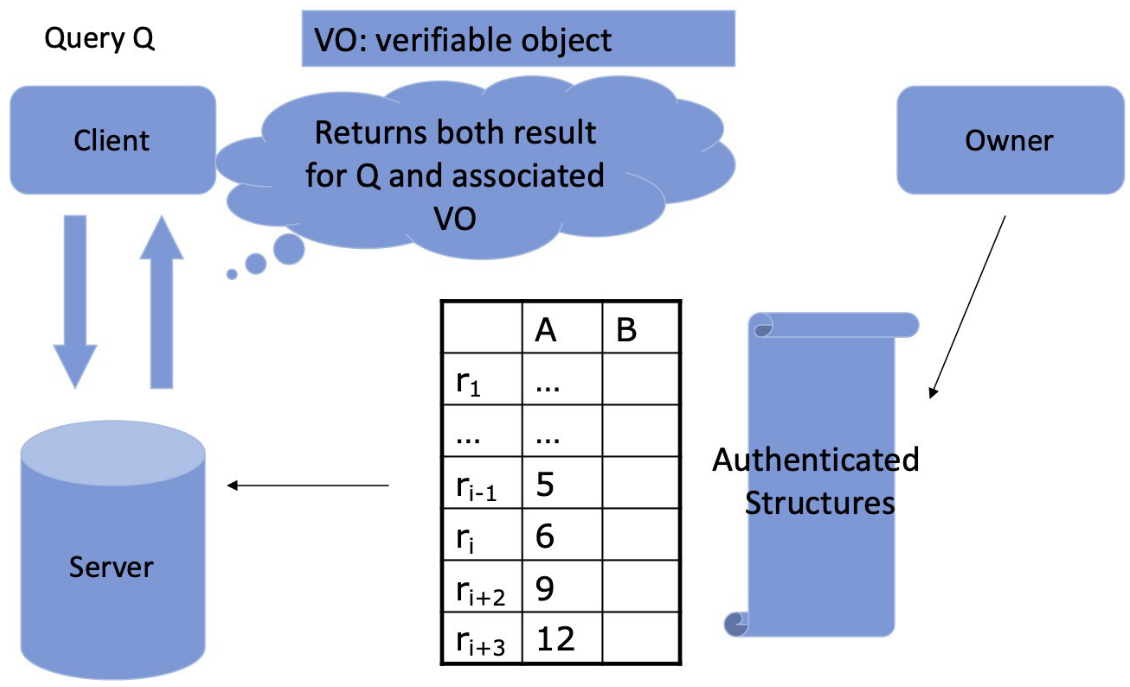
\includegraphics[width=0.8\linewidth]{images/det-idea.png}
\end{figure}

\section{Approccio basato su firma}

Questa tecnica si preoccupa di verificare l'integrità solo per una tipologia
particolare di query, ovvero quelle che coinvolgono un solo attributo 
della relazione; ad esempio $x=5, 4<x<5,\dots$ l'idea è:
\begin{itemize}
    \item ordinare le tuple rispetto al valore dell'attribuo preso in considerazione 
    \item applicare una firma alle tuple, non singolarmente ma in coppie tra loro consecutive 
    
    $(t_1,s_1),(t_2,s_2)\dots(t_n,s_n), con s_i = \epsilon(t_i | t_{i+1})$ 
    \item oltre ai dati, vengono date al provider anche le firme
\end{itemize}

\noindent A questo punto quando un client vuole eseguire una computazione, ad esempio 
$a<x<b$:
\begin{itemize}
    \item vengono restituite le tuple (e le firme associate) $[a-1,b+1] \rightarrow$ voglio anche la tupla 
    immediatamente precedente ed immediatamente successiva 
    \item le \textit{cose aggiunte} al risultato vero e proprio per verificare l'integrità sono: 
    \begin{itemize}
        \item tuple precedente e successiva 
        \item firme associate alle tuple 
    \end{itemize}
\end{itemize} 

\noindent $\Rightarrow$ l'idea è che il client tramite le firme può verificare se il risultato è integro.

\noindent Questo metodo non è molto utilizzato perché:
\begin{itemize}
    \item limitazione sulle query
    \item costosa sia in termini di computazione delle firme, sia nei termini di informazioni 
    aggiuntive che ti devo dare (lineare rispetto al risultato)
\end{itemize}

\begin{figure}[H]
    \centering
    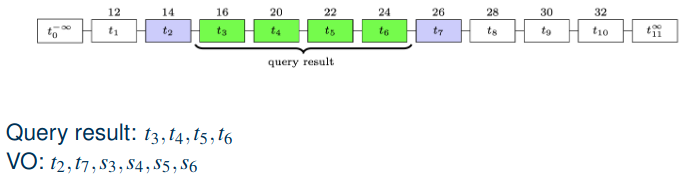
\includegraphics[width=1\linewidth]{images/signature.png}
    \caption{VO sta per verification object}
\end{figure}


\newpage
\section{Merkle hash tree}
Questa tecnica può essere utilizzata per risolvere lo stesso tipo di query viste 
nella sezione precedente, ma in maniera più efficiente. 

\begin{figure}[H]
    \centering
    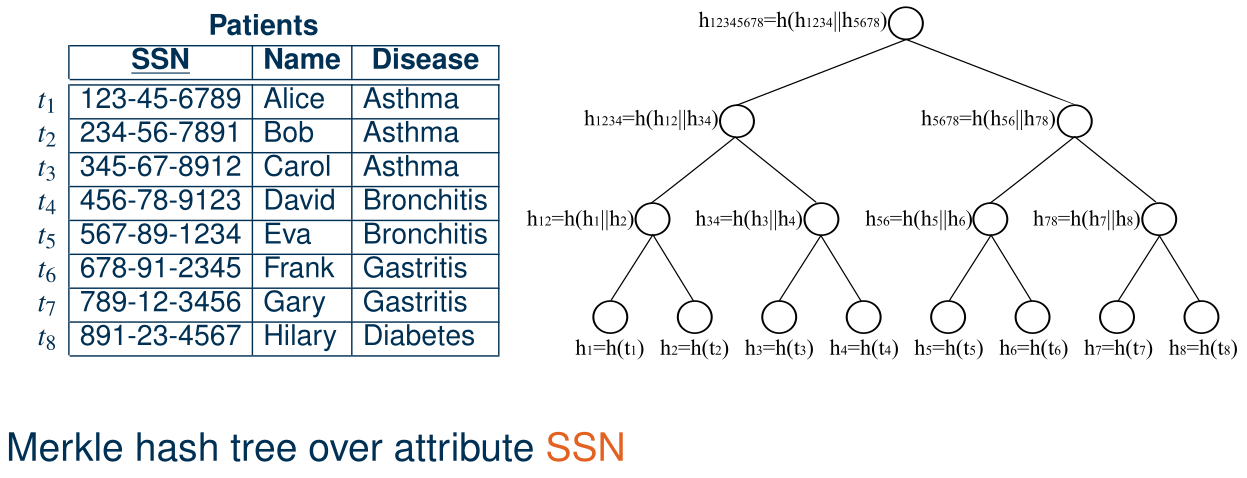
\includegraphics[width=1\linewidth]{images/merkle-hashtree.png}
\end{figure}

L'idea è:
\begin{itemize}
    \item ordinare i valori dell'attributo preso in considerazione
    \item si applica una funzione di hash alle tuple (foglie dell'albero)
    \begin{itemize}
        \item nel livello delle foglie ci sono $2^L$ elementi
        \item i nodi intermedi vengono calcolati applicando la stessa funzione di hash 
        alla concatenazione degli hash dei figli 

        \noindent $\rightarrow$ l'idea è che l'hash di un nodo dipende dall'hash dei figli
        \item se l'albero non è completo, tipicamente si aggiungono delle tuple \textit{null} per renderlo completo 
    \end{itemize}
\end{itemize}

$\Rightarrow$ la quantità di informazioni aggiuntive non è più lineare rispetto al risultato 
ma è \textbf{logaritmica}.

\subsection{Merkle hash tree verification}

\begin{itemize}
    \item L'idea è che il cloud provider fornisce un \textit{\textbf{verification object}} per 
    permettere al client di \textbf{ricostruire l'hash associato alla radice}
    \item Il risultato della query è \textbf{corretto e completo} la radice calcolata 
    corrisponde a quella già conosciuta
    \begin{itemize}
        \item se c'è una tupla mancante o non corretta, la radice calcolata sarà diversa da quella già conosciuta
    \end{itemize}
\end{itemize}

\begin{figure}[H]
    \centering
    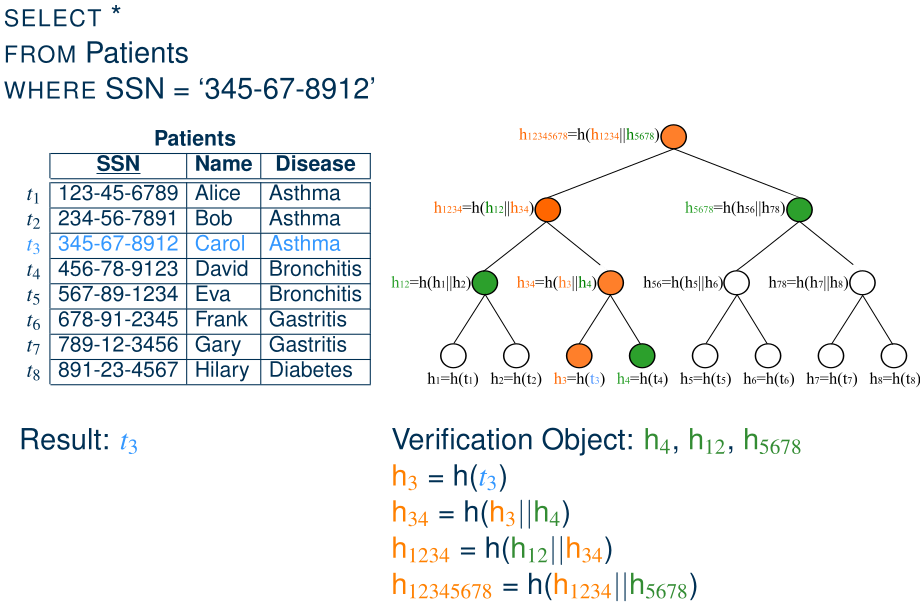
\includegraphics[width=1\linewidth]{images/tree-verification.png}
\end{figure}

\begin{figure}[H]
    \centering
    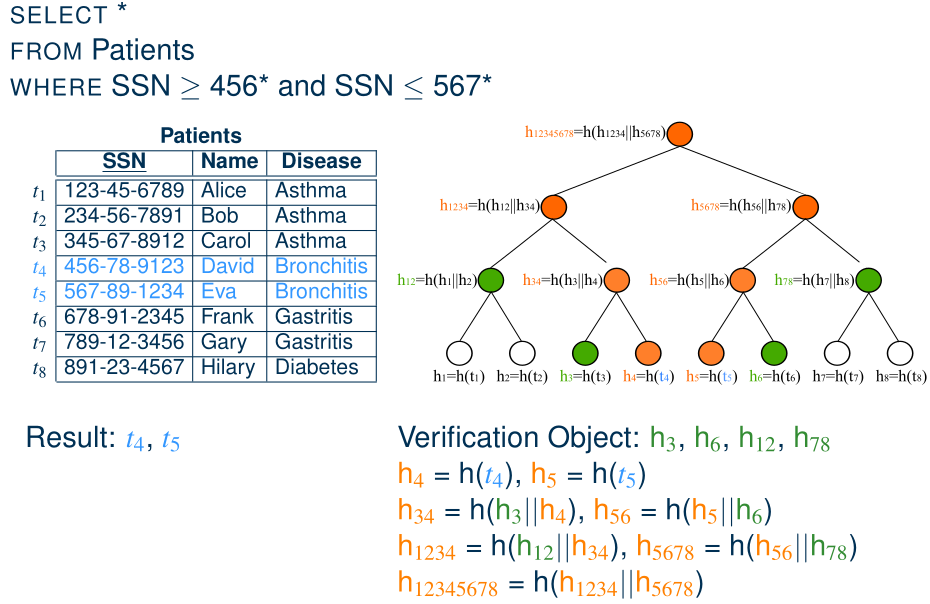
\includegraphics[width=1\linewidth]{images/tree-verification2.png}
\end{figure}

\noindent Con la tecnica delle firme, il costo della verifica è lineare rispetto alla dimensione del risultato; mentre 
con la tecnica dell'albero il costo è sempre pari a $\log n$ (\textit{n numero di foglie})

$\rightarrow$ quando la dimensione del risultato supera $\log n$, sarà più efficiente usare l'albero

\section{Merkle B-tree}
Ciascun nodo contiene più informazioni:
\begin{itemize}
    \item Nodo foglia:
    \begin{itemize}
        \item chiave $k_i$
        \item puntatore all'area di memoria che contiene l'informazione vera e propria 
        \item funzione di hash applicata alla tupla con chiave $k_i$
    \end{itemize}
    \item Nodo interni:
    \begin{itemize}
        \item chiave
        \item puntatori ai nodi figli 
        \item funzione di hash applicata alla concatenazione di tutti gli hash che appaiono nel nodo puntato dal puntatore
    \end{itemize}
\end{itemize}

\begin{figure}[H]
    \centering
    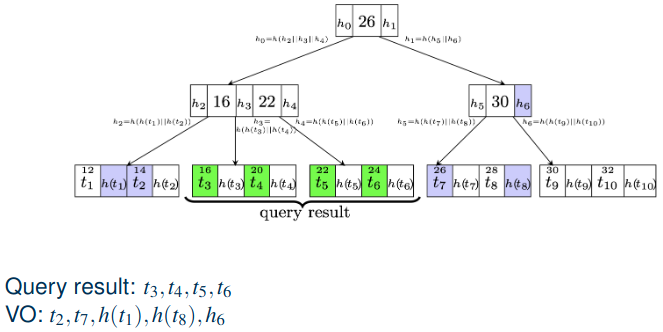
\includegraphics[width=1\linewidth]{images/mb-tree}
\end{figure}

\noindent Per semplicità la tupla nei nodi foglia è memorizzata direttamente all'interno del nodo.

\noindent Concettualmente il meccanismo di funzionamento e verifica è lo stesso dell'albero visto precedentemente; possiamo vedere 
questa versione come una sua generalizzazione in cui ogni nodo può contenere più chiavi.
\begin{itemize}
    \item l'hash associato al nodo radice è un \textit{summary} di tutte le informazioni che contiene l'albero 
\end{itemize}




\section{Skip list}
Ha lo svantaggio che può essere usata solo con query di uguaglianza, ma ha il vantaggio 
di poter essere integrata in modo efficiente in un DBMS.

\noindent Una \textbf{skip list} è una lista



\begin{itemize}
    \item Una \textbf{skip list} per un set di elementi è una serie di liste $S_1, S_2, \dots, S_n$, tale che:
    \begin{itemize}
        \item $S_0$ contiene tutti gli elementi ordinati rispetto a un qualche attributo e le sentinelle $+\infty$ e $-\infty$
        \item $S_i$ contiene un sottoinsieme degli elementi della lista $S_{i-1}$ con una probabilità $p$ (le sentinelle sono sempre inlcuse)
    \end{itemize}
    \item Ha il vantaggio che tutte le operazioni vengono fatte in tempo $O(log(n))$, per cui è molto efficiente
    \begin{itemize}
        \item \texttt{find(x)}
        \item \texttt{delete(x)}
        \item \texttt{insert(x)}
    \end{itemize}
\end{itemize}

\subsection{Search operation}
\begin{itemize}
    \item Si inizia dall'elemento sentinella nella top list ($-\infty$ nella lista più in alto)
    \item Vado avanti finché trovo un valore $\leq$ di quello che sto cercando (\textit{hop forward})
    \item Nel caso in cui ce ne fosse uno maggiore, allora scendo nella lista sotto (\textit{top down}) e proseguo 
    la ricerca con lo stesso procedimento
\end{itemize}

\begin{figure}[H]
    \centering
    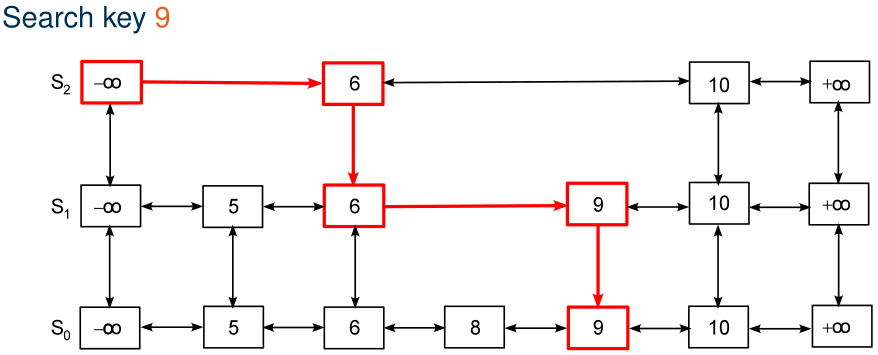
\includegraphics[width=1\linewidth]{images/skip-list.png}
\end{figure}

\subsection{Authenticated skip list}

\noindent Ad ognuno dei nodi si applica una funzione di hash $h$:
\begin{itemize}
    \item resistente a collisioni 
    \item commutativa ($h(x,y)=h(y,x)$)
\end{itemize}

\noindent Ad ogni nodo viene associata una etichetta che, insieme ai \textit{verification object}, permettono di ricostruire il cammino della ricerca 
nel senso opposto, allo scopo di verificare la computazione.

\begin{figure}[H]
    \centering
    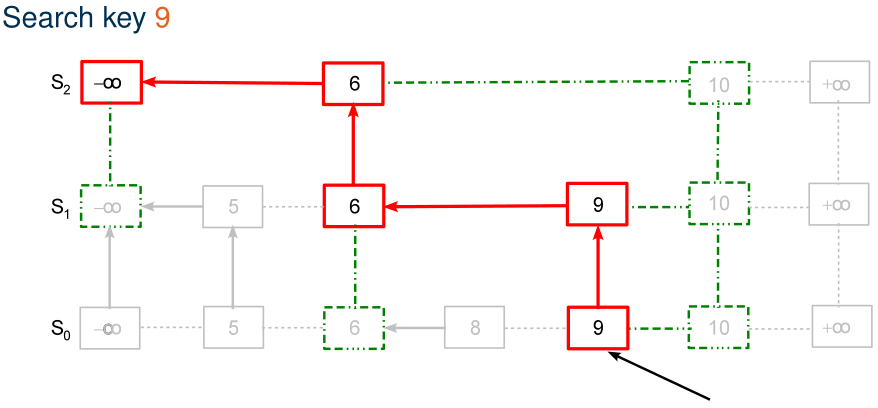
\includegraphics[width=1\linewidth]{images/skip-list-auth.png}
\end{figure}



\chapter{Approcci probabilistici}
Lo svantaggio è che non si ha più la certezza sui risultati, ma hanno il vantaggio di coprire 
più tipologie di query. 


\section{Introduzione}
Possono essere usate due tecniche principali, che possono essere combinate tra loro 
per ottenere una maggiore efficacia.

\subsection{Fake tuples}
L'idea è mettere dentro ai dati originali dei dati fasulli e li mischio; dopo posso controllare 
la loro presenza nel risultato della query (al client restituisco anche le tuple fasulle, lui 
controllerà che ci sono tutte le tuple fasulle che si aspetta).

\noindent Questo meccanismo ha una serie di problematiche che devono essere affrontate:
\begin{itemize}
    \item le tuple \textit{fake} \textbf{non devono essere riconoscibili} da quelle reali 
    \item si utilizzano \textbf{dati criptati} per proteggerli (questo ci aiuta nel punto precedente)
    \item si associa a ciascuna tupla una \textit{informazione aggiuntiva} per verificare l'\textbf{autenticità dei dati}; posso 
    pensare di applicare una funzione di hash alla concatenazione dei valori degli attributi della tupla; questa informazione aggiuntiva 
    la uso anche per distinguere le tuple fasulle da quelle originali
\end{itemize}

\subsubsection{Approccio random}
Quando il client ottiene il risultato di una query, poi deve filtrare le tuple fasulle facendo una 
ulteriore query in locale

$\Rightarrow$ \textcolor{red}{\textbf{il client deve tenersi una copia delle tuple fasulle e computare una query}}

\noindent\dots bisogna pensare ad un altro approccio più efficiente

\subsubsection{Approccio determinstico}
Viene tenuta localmente la funzione usata per generare le tuple fasulle (al posto delle tuple 
fasulle); per semplificare il passo di verifica, l'idea è:
\begin{itemize}
    \item si partizionano i domini
    \item per ogni partizione mi segno quante tuple fasulle gli appartengono 
    \item quando eseguo una query, saprò se una certa partizione del dominio sarà \textit{coperta} parzialmente o completamente dal risultato della query
    \item per verificare farò il conteggio delle tuple fasulle 
\end{itemize}


\begin{figure}[H]
    \centering
    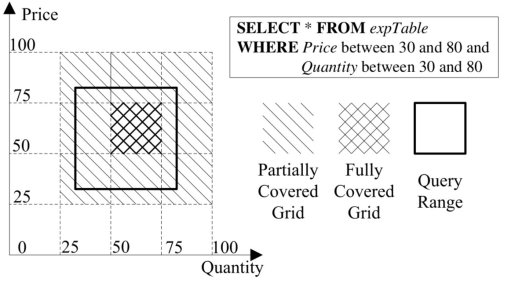
\includegraphics[width=0.8\linewidth]{images/fake-tuples.png}
\end{figure}

\noindent Per calcolare il numero di tuple in una determinata sezione, io conosco 
la funzione usata per generare le tuple; per cui mi basta calcolare i punti 
di intersezione per fare il conteggio (è importante che la funzione sia monotona).

\begin{figure}[H]
    \centering
    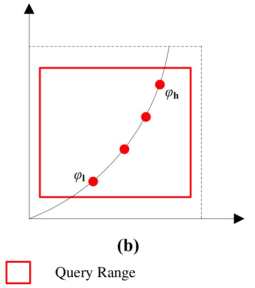
\includegraphics[width=0.4\linewidth]{images/fake-tuples-1.png}
\end{figure}


\subsection{Duplicazione di tuple}
L'idea è quella di non usare tuple fake ma di duplicare alcune tuple reali; la verifica viene 
fatta contando il numero di tuple doppie che mi aspetto di avere. 


\section{Computazione con provider multipli}
Lo scenario di riferimento è quello con multiple sorgenti informative; supponiamo che le 
entità che hanno in mano i dati siano fidate, ma che le computazioni (magari perché sono 
costose) vengano fatte sfruttando le risorse computazionali di qualcun'altro (costa meno 
rispetto a gestirle direttamente).

\noindent Questa entità che gestisce le computazioni non è fidata; anzi, meno costa probabilmente 
meno è fidata \dots devo verificare il risultato che viene restituito.

\noindent In questo contesto vengono combinate le tecniche viste in precedenza.

\begin{figure}[H]
    \centering
    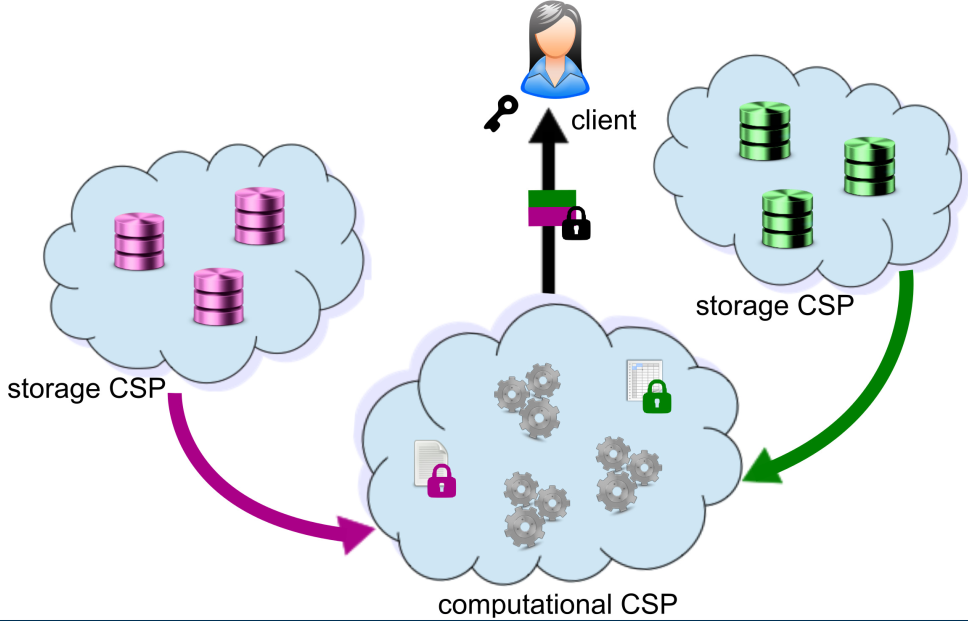
\includegraphics[width=0.8\linewidth]{images/scenario.png}
\end{figure}

\section{Approccio probabilistico per query di join}
Questo tipo di query è quello tipicamente più costoso; le tecniche di protezione 
sono:
\begin{itemize}
    \item \textbf{dati criptati}: proteggo i dati criptandoli perché non mi fido dell'entità che esegue la computazione
    \item \textbf{markers} (tuple fake): prima di consegnarli aggiungo tuple fasulle
    \item \textbf{twins} (tuple replicate): prima di consegnarli replico alcune tuple
    \item \textbf{salts/buckets}: voglio evitare che chi prende i miei dati (a cui ho aggiunto le informazioni di controllo)
    non deve essere in grado di distinguere le informazioni di controllo dai dati veri e propri
\end{itemize}


\noindent L'idea è:
\begin{itemize}
    \item ho due storage server che sono fidati e che hanno in mano i dati veri e propri
    \item ciascuno dei due server mette dentro \textit{markers} e \textit{twins}
    \item criptano i dati e li danno a \textit{qualcun'alro (computational cloud)}, che non è più 
    grado di distinguere i dati veri da quelli spuri
    \item viene fatta la operazione di join 
    \item chi ha richiesto l'esecuzione della query decripta il risultato, fa tutte le verifiche opportune 
    (markers e twins) e si tiene il risultato
\end{itemize}

\begin{figure}[H]
    \centering
    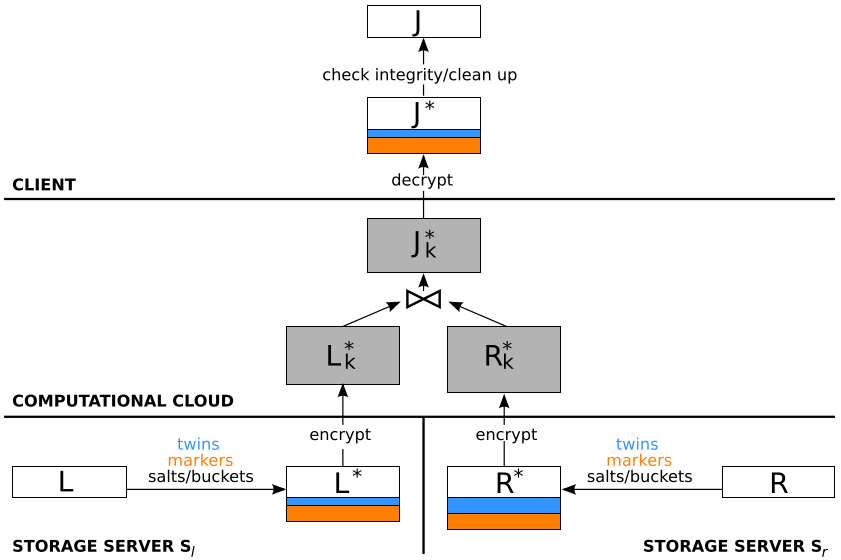
\includegraphics[width=1\linewidth]{images/join.png}
\end{figure}

\subsection{On-the-fly encryption}
Devo criptare separatamente ogni attributo di join per proteggerli (gli altri attributi 
al computational cloud non interessano\dots anche se li cripto tutti insieme va bene lo stesso).

\noindent Il client genera la chiave di criptazione che viene comunicata agli storage server tramite il 
computational cloud; gli storage server utilizzano questa chiave per criptare separatamente:
\begin{itemize}
    \item attributo di join 
    \item tutti gli altri attributi 
\end{itemize}

\noindent Danno queste relazioni criptate al computational cloud che computerà il join 
(è importante affinché il computational cloud possa eseguire il join che i server usino la stessa chiave).

\begin{figure}[H]
    \centering
    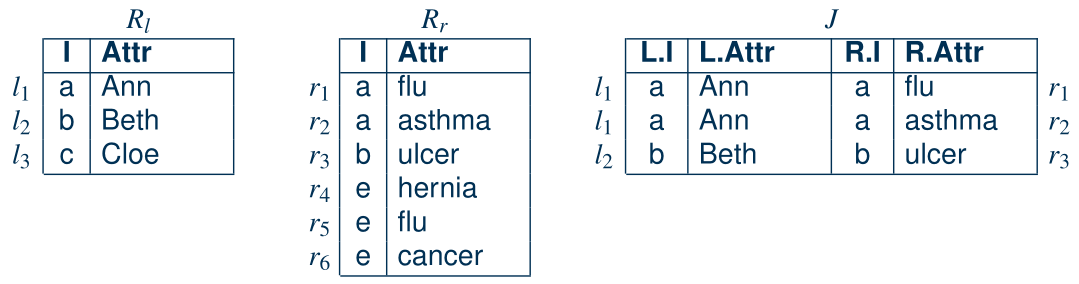
\includegraphics[width=1\linewidth]{images/otf1.png}
\end{figure}

\begin{figure}[H]
    \centering
    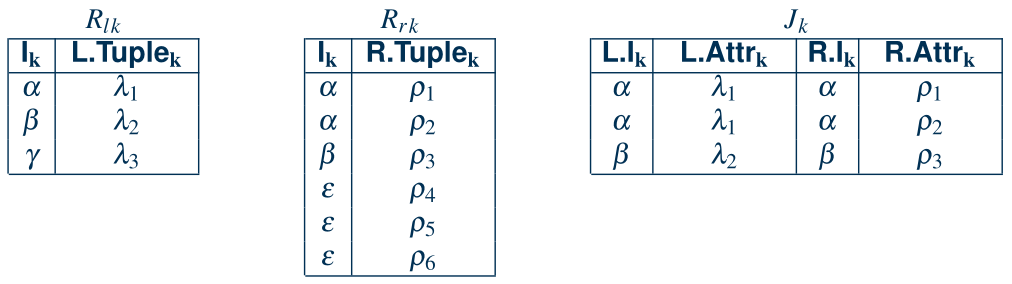
\includegraphics[width=1\linewidth]{images/otf2.png}
\end{figure}



\subsection{Markers}

Gli storage server iniettano delle tuple fasulle; dato poi il computational cloud lavora sul criptato, non 
mi devo neanche preoccupare di generare delle tuple \textit{simili al vero}.

\noindent Tuttavia, per gli attributi di join il valore deve essere generato con attenzione, perché 
voglio evitare che tuple fasulle si combinino con tuple vere; devo avere la garanzia che 
quel valore possa essere un valore reale per l'attributo di join.

\begin{figure}[H]
    \centering
    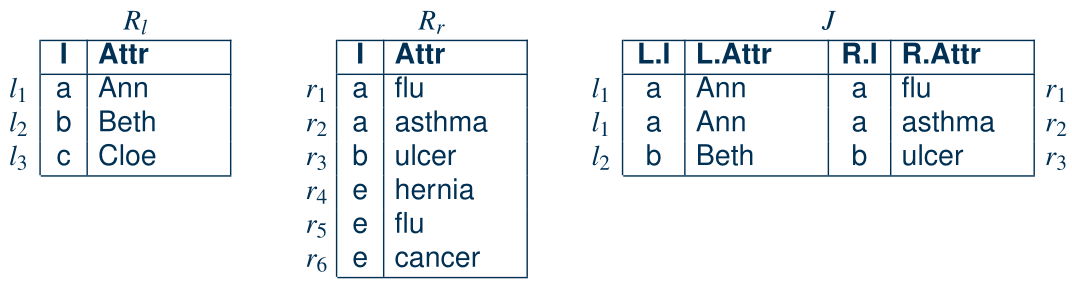
\includegraphics[width=1\linewidth]{images/marker1.png}
\end{figure}

\begin{figure}[H]
    \centering
    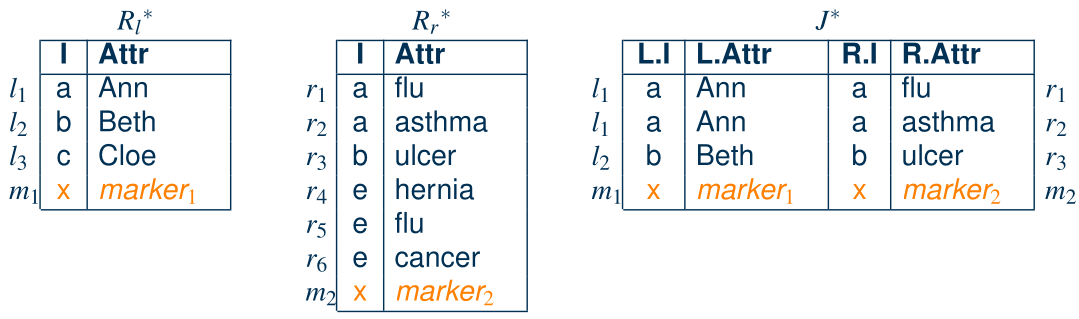
\includegraphics[width=1\linewidth]{images/marker2.png}
\end{figure}


\noindent Ad esempio, per avere certezza che non ci sia mai questa collisione, potrei:
\begin{itemize}
    \item combinare i valori veri con un certo $v$
    \item combinare i valori fasulli con un valore distinto $v'$
\end{itemize}

\noindent Devo sostanzialmente inventarmi un qualunque meccanismo che mi assicuri che non ci sia collisione.

\subsection{Twins}

Gli storage server (senza coordinarsi, neanche si conoscono \dots) duplicano alcune tuple;
il problema è: \textit{quali tuple vado a duplicare?}

\noindent Gli storage server devono duplicare le tuple in modo tale che queste tuple si combinino 
correttamente durante la operazione di join; mi devo trovare queste tuple duplicate nel risultato del join, 
altrimenti non avrebbe senso.

$\Rightarrow$ \textbf{devono duplicare le tuple con lo stesso attributo di join}

\noindent L'unico modo per avere 
questa garanzia senza che i server comunichino tra loro, il client comunica quali tuple devono essere 
duplicate; ad esempio, tutte le tuple che soddisfano una certa condizione che dipende dall'attributo di join).

\begin{figure}[H]
    \centering
    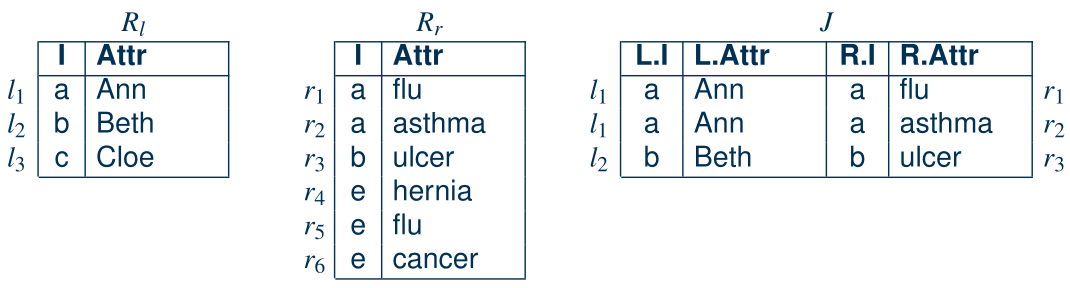
\includegraphics[width=1\linewidth]{images/twins1.png}
\end{figure}

\begin{figure}[H]
    \centering
    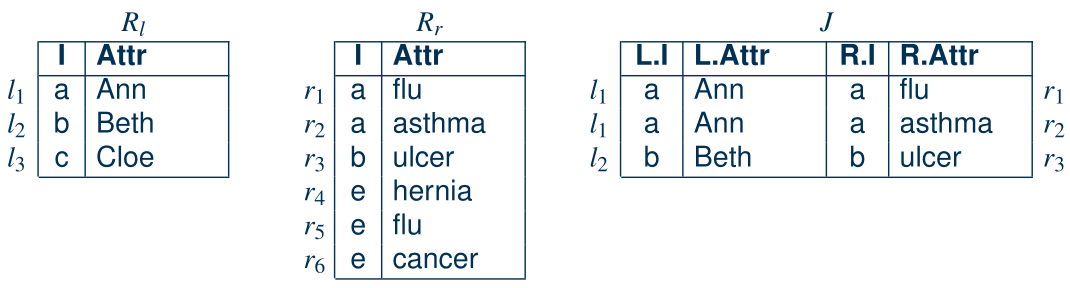
\includegraphics[width=1\linewidth]{images/twins1.png}
\end{figure}



\subsection{Salts and buckets}

Cercano di eliminare le \textbf{frequenze riconoscibili} delle combinazioni in 
join \textit{one-to-many}. 

\noindent Il problema sta nella tabella con molte tuple (\textit{many}):
\begin{itemize}
    \item se una tupla ha 1 sola occorrenza, potrei inferire che si tratta di un marker, dato che vengono 
    generati con valori (per l'attributo di join) sempre diversi per evitare collisioni (non ho la certezza, ma 
    sospetta che possa essere un marker)
    \item se ho tuple con lo stesso valore ripetuto per l'attributo di join, allora inferisco che sicuramente non 
    sono marker; non possono nemmeno essere twins perchè vanno sempre a coppie (multipli di 2); quindi capisco che sono tuple vere
\end{itemize}


\noindent Questi attacchi sfruttano la frequenza con cui appaiono i valori degli attributi di join; 
per evitarli si cerca di appiattire queste frequenze, ovvero tutti i valori possibili appaiono tutti con la medesima 
frequenza; viene fatto in due modi:
\begin{itemize}
    \item \textbf{Sali:} si combinano i valori dell'attributo di join con un valore casuale
    \begin{itemize}
        \item ha lo svantaggio che la tabella \textit{one} aumenta di dimensione per appiattire la frequenza delle occorrenze
        \item ha il vantaggio che la dimensione del risultato del join rimane invariata
    \end{itemize}
    \item \textbf{Bucket:} creo dei gruppi di tuple, dove tutte le tuple appartenenti ad un bucket 
    hanno lo stesso valore per l'attributo di join
    \begin{itemize}
        \item devo aggiungere delle tuple \textit{dummy} nella tabella \textit{many} per ottenere 
        la dei gruppi con dimensione uniforme 
        \item i join non saranno $(1:1)$ ma saranno tutti con la stessa frequenza, quindi non posso inferire nulla 
        \item lo svantaggio è che aumenta la dimensione sia della tabella \textit{many} che del risultato del join 
    \end{itemize}
\end{itemize}

\begin{figure}[H]
    \centering
    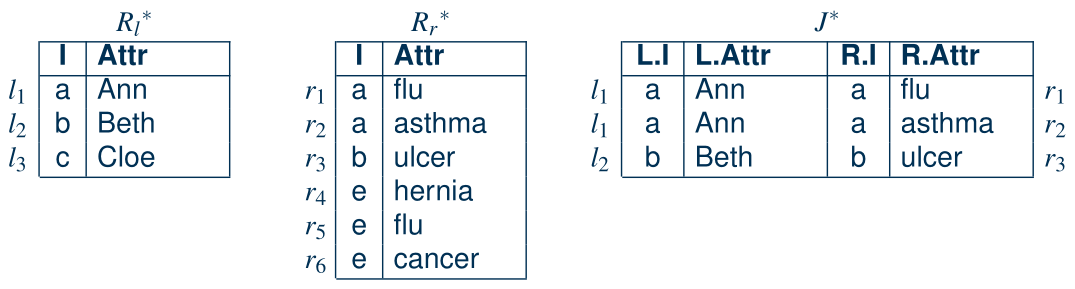
\includegraphics[width=1\linewidth]{images/salt1.png}
\end{figure}

\begin{figure}[H]
    \centering
    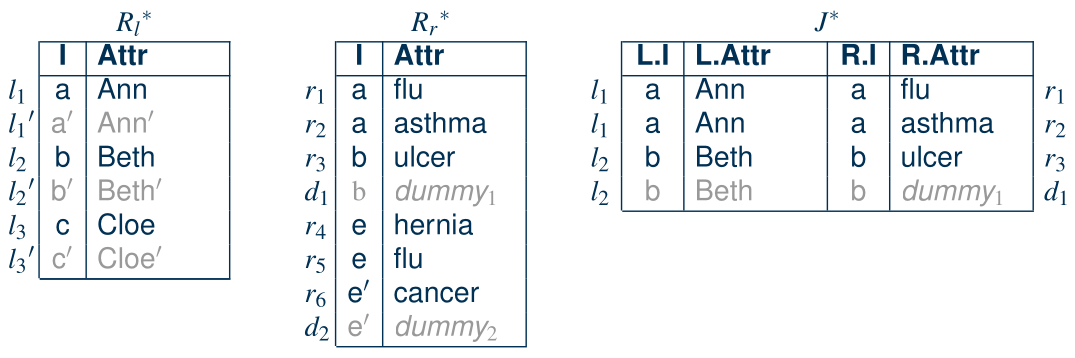
\includegraphics[width=1\linewidth]{images/salt2.png}
\end{figure}

\noindent Le tecniche di \textit{salt} e \textit{bucket} possono essere 
usate sia singolarmente che in combinazione.


\subsection{Valutazione delle query}

Il client:
\begin{itemize}
    \item parla con colui che esegue la query (computational cloud), non con i server; gli manda 
    la richiesta di join e quali sono i server da coinvolgere 
    \item tra le varie informazioni che il client manda al cloud, ci sono:
    \begin{enumerate}
        \item Sotto-query che ciascun server deve eseguire sulla sua tabella
        
        \texttt{SELECT * FROM L, R}
        
        \texttt{WHERE L.Name = R.Name and \hl{L.Stipendio > 1000}}

        \item Chiave di criptazione della query
        \item Numero di marker da iniettare
        \item Percentuale di twins 
        \item Numero di sali da utilizzare
    \end{enumerate}

    \noindent Tutte queste informazioni protette vengono criptate con la chiave pubblica degli storage server per passarle al cloud (\textit{honest-but-curious}).
\end{itemize}

\begin{figure}[H]
    \centering
    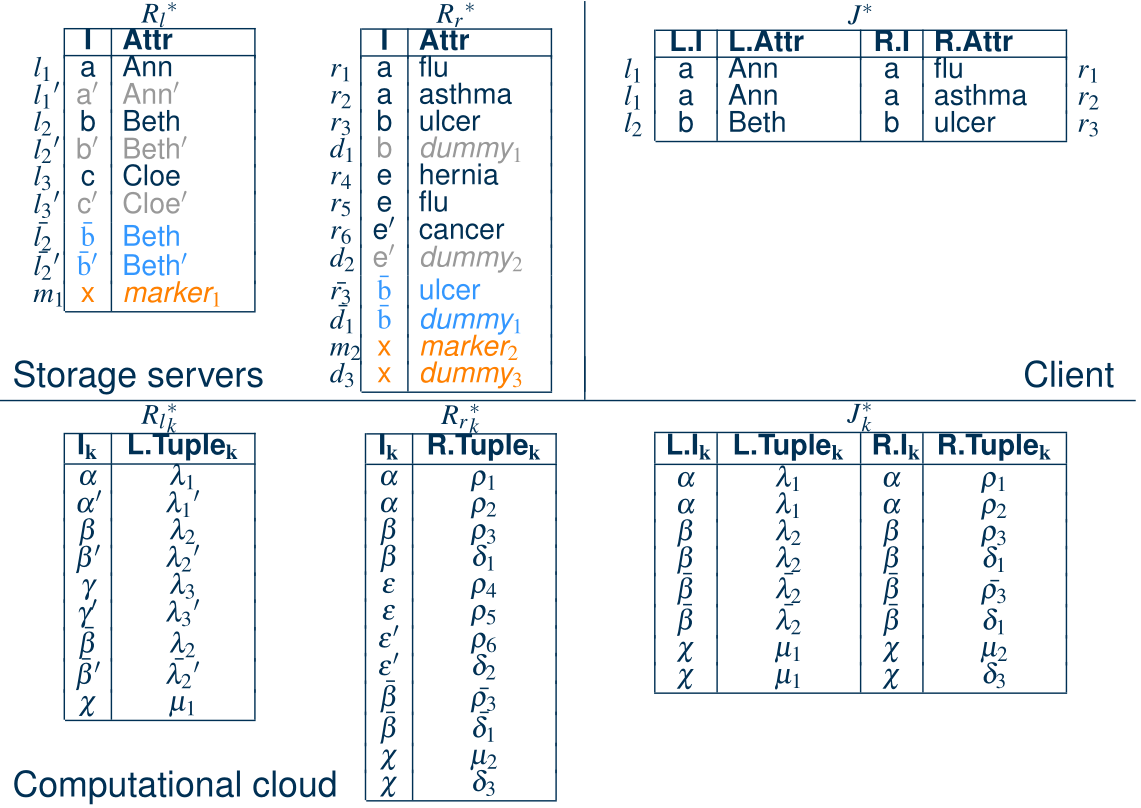
\includegraphics[width=1\linewidth]{images/join-execution.png}
\end{figure}

\subsection{Markers e twins: garanzia dell'integrità}

I markers e twins offrono una protezione complementare; senza la loro combinazione potrebbero 
rimanere scoperti alcuni casi estremi:
\begin{itemize}
    \item i \textbf{twins sono efficaci il doppio}, ma perdono la loro efficacia quando il computational cloud 
    omette una grande parte delle tuple (caso estremo: omette tutte le tuple)
    \begin{itemize}
        \item \textit{se butto via poco, mi proteggono bene i twins perché dovrei avere la fortuna di buttare via entrambi i twins}
    \end{itemize}
    \item i \textbf{markers permettono di rilevare casi estremi}
\end{itemize}

\section{Semi-join}
Protegge il join:
\begin{itemize}
    \item senza introdurre salts e buckets 
    \item supporta \textit{one-to-one, one-to-many, many-to-many}
\end{itemize}

Dato che il problema è la frequenza delle occorrenze dei valori di join, si proietta tutto su 
di essi: 
\begin{enumerate}
    \item \texttt{SELECT Name WHERE I=A}
    \item \texttt{SELECT DoB WHERE I=A}
    \item si fa il \textit{merge} dei risultati ottenuti 
\end{enumerate}

\noindent Proiettando tutto sull'attributo di join, avrò solo una occorrenza 
dei valori di join; in questo modo sto automaticamente appiattendo le frequenze.
\begin{itemize}
    \item Ha il vantaggio di non aumentare la dimensione delle tabelle 
    \item Ha lo svantaggio che il client deve si prende in carica contattare i server e 
    di calcolare i risultati; non gli viene dato già pronto
\end{itemize}



\section{Computational cloud distribuito}
Il computational cloud non è un'unica entità, ma in questo scenario è distribuito; ci sono più nodi, 
ciascuno prende una parte della relazione per computare la sua parte, ed infine il risultato 
viene messo insieme.

\noindent  il problema è verificare se il risultato ottenuto combinando i risultati parziali 
va bene o no

$\Rightarrow$ \textbf{ho il problema di come distribuire le informazioni di controllo}

\subsection{MapReduce}

È un framework distribuito con più nodi (\textit{workers}) basato su due funzioni:
\begin{itemize}
    \item \textbf{Map:} definita lato client, ha l'obiettivo di trasformare i dati su cui vogliamo eseguire una computazioni in un insieme di coppie 
    \begin{itemize}
        \item il primo campo è una chiave 
        \item il secondo campo è il valore
    \end{itemize}
    \item \textbf{Assignement:} una funzione di assegnamento che assegna delle coppie ai workers; le coppie con la stessa 
    chiave appartengono allo stesso worker
    \item \textbf{Reduce:} funzione eseguita da ciascun worker che produce il risultato parziale
\end{itemize}


\noindent Ogni worker esegue la sua funzione di reduce; successivamente, il \textit{manager} combina i vari risultati parziali 
per ottenere il risultato finale.

\subsection{On-the-fly encryption}
Dato che non ci fidiamo del computational cloud, 
vengono create delle coppie criptate, dove:
\begin{itemize}
    \item la chiave è il valore dell'attributo criptato 
    \item il valore è il nome della relazione a cui appartiene 
\end{itemize}


\subsection{Markers and MapReduce}




















\end{document}